% WACV 2027 Paper Draft
\documentclass[10pt,twocolumn,letterpaper]{article}

\usepackage[review,datasets]{wacv}

\usepackage{times}
\usepackage{epsfig}
\usepackage{graphicx}
\usepackage{amsmath}
\usepackage{amssymb}
\usepackage{booktabs}
\usepackage{multirow}
\usepackage{array}
\usepackage{xcolor}

\definecolor{wacvblue}{rgb}{0.21,0.49,0.74}
\usepackage[pagebackref,breaklinks,colorlinks,allcolors=wacvblue]{hyperref}

\def\wacvPaperID{*****}
\def\confName{WACV}
\def\confYear{2027}

\newcommand{\method}{RidgeLoRA-FP}
\newcommand{\TODO}[1]{\textcolor{red}{[TODO: #1]}}

\title{\method: Lightweight Ridge-Conditioned Fingerprint Diffusion for Affordable Cross-Sensor Synthetic Data}

\author{
Anonymous WACV submission\\
Paper ID *****}

\begin{document}
\maketitle

\begin{abstract}
Synthetic fingerprint data can reduce the cost and privacy burden of training
fingerprint recognition systems, but useful synthetic data must satisfy two
constraints at once: it must preserve identity-discriminative ridge and minutiae
structure, and it must cover the sensor-dependent appearance shifts that occur
in operational deployments.  We present \method, a lightweight two-stage latent
diffusion pipeline for generating multi-sensor fingerprint impressions.  Stage
1 samples a fingerprint identity in a compressed VQ-VAE latent space .  Stage 2 turns the generated identity into multiple
sensor-specific impressions using a ridge-conditioned generator, pose-mask
alignment, and small control perturbations.  For adapting to a new sensor, we
freeze the identity model and the ridge-control path and fine-tune only LoRA
weights in the Stage-2 denoising UNet.  This design targets affordable
research hardware: the base denoiser is compact, sampling uses DDIM in latent
space, and a sensor adapter is a small LoRA checkpoint rather than a full
diffusion model.  We use FPGAN-Control as the primary competitor on NIST
SD302A, and treat SD301A, SD302B, and FVC-style sensor transfer as new
cross-sensor settings enabled by the proposed conditioning and adapter design.
\end{abstract}

\section{Introduction}
\label{sec:introduction}

Fingerprint recognition research is constrained by the scarcity of public,
large-scale, multi-impression datasets.  Unlike generic image classification,
the training data must represent both identity-level structure, such as ridge
flow and minutiae configuration, and acquisition-level variation, such as
sensor noise, contrast, pressure, cropping, pose, and background artifacts.
Collecting such data is expensive and privacy-sensitive, and the resulting
datasets are often too small for training robust deep recognizers.

Recent fingerprint generators address this gap by synthesizing multiple
impressions of each synthetic finger.  FPGAN-Control~\cite{shoshan2023fpgan}
is the closest baseline for our setting because it is trained and evaluated on
NIST SD302/N2N and explicitly controls fingerprint appearance.  GenPrint
\cite{grosz2024genprint} extends the direction to a much broader multimodal
latent-diffusion framework with text and image conditions, but its reported
training recipe uses a Stable-Diffusion-scale model, 500k LoRA steps, and 8
A100 GPUs.  That level of compute is not always available to smaller
biometrics labs that want to prototype recognition models on commodity GPUs
such as an NVIDIA RTX A4000.

This work explores a more pragmatic point in the design space.  Rather than
fine-tuning a large general-purpose text-to-image model, \method uses a compact
fingerprint-specific latent diffusion model.  Sensor appearance is represented
by a ConvNeXt descriptor pooled from a small set of reference images from the
target sensor.  Identity preservation is handled through an explicit ridge
condition in the second stage.  Finally, sensor adaptation is performed with
Stage-2 UNet LoRA only: the first-stage identity generator and the structural
control path remain frozen.

Our contributions are:
\begin{itemize}
    \item A lightweight sensor-conditioned latent diffusion pipeline for
    generating fingerprint identities and multi-sensor impressions.
    \item A Stage-2 ridge-conditioned synthesis module with pose-mask alignment
    and mild control augmentation, reducing over-constrained pose transfer from
    the source identity ridge.
    \item A parameter-efficient sensor adaptation protocol that fine-tunes only
    LoRA weights in the Stage-2 denoising UNet.
    \item An evaluation plan centered on SD302A comparison to FPGAN-Control,
    with SD301A, SD302B, and FVC-style sensors used as cross-sensor
    generalization contributions rather than additional baseline comparisons.
\end{itemize}

\section{Related Work}
\label{sec:related}

\paragraph{Synthetic fingerprints.}
Classical systems such as SFinGe~\cite{cappelli2002synthetic} construct
fingerprints using hand-designed ridge flow, shape, and noise models.  Recent
GAN-based methods improve realism and scale.  PrintsGAN~\cite{engelsma2022prints}
generates large sets of synthetic fingers with multiple impressions per finger,
which is essential for training embedding-based recognizers.  FPGAN-Control
\cite{shoshan2023fpgan} further disentangles identity and appearance factors,
allowing image appearance attributes such as sensor and pressure to be varied
while keeping identity fixed.  Because FPGAN-Control is evaluated on the NIST
SD302/N2N setting, we use it as our main competitor.

\paragraph{Fingerprint diffusion.}
Latent diffusion models reduce pixel-space diffusion cost by denoising in a
compressed latent representation~\cite{rombach2022ldm}.  GenPrint
\cite{grosz2024genprint} applies a multimodal latent diffusion model to
fingerprints, using text prompts and image style embeddings to control
acquisition type, sensor, quality, and identity.  GenPrint is a strong
reference point for universality, but it is built on a larger Stable
Diffusion-style backbone and a broad multi-dataset training recipe.  Our goal
is complementary: provide a smaller, faster pipeline that can be trained,
sampled, and adapted by recognition teams with modest hardware.

\paragraph{Structural control and efficient adaptation.}
ControlNet~\cite{zhang2023controlnet} adds trainable control branches to a
frozen diffusion model for spatially aligned conditions.  For fingerprints,
ridge maps are a natural structural condition because they encode the ridge
flow and minutiae layout used by matchers.  LoRA~\cite{hu2022lora} provides a
low-rank adaptation mechanism for fine-tuning large neural networks with few
trainable parameters.  DataDream~\cite{kim2024datadream} demonstrates the
usefulness of example-guided LoRA adaptation for dataset generation.  We adapt
this idea to fingerprint sensors by tuning only Stage-2 UNet LoRA weights.

\section{Method}
\label{sec:method}

\subsection{Overview}

\method is a two-stage generator.  Stage 1 samples a synthetic fingerprint
identity.  Stage 2 renders multiple impressions of that identity under target
sensor appearances.  Both stages operate on $512 \times 512$ grayscale images
encoded into $128 \times 128 \times 3$ VQ-VAE latents.  The VQ-VAE is frozen.

Let $x$ be a fingerprint image, $z=E(x)$ its latent, and $s$ a sensor style
condition.  Stage 1 models $p_\theta(z \mid s)$ and generates a base identity
image $\hat{x}^{id}$.  A ridge extractor produces a control map
$r = R(\hat{x}^{id})$.  Stage 2 then samples impressions
$\hat{x}^{imp}_1,\ldots,\hat{x}^{imp}_K$ conditioned on both the ridge map and
the target sensor style.

\subsection{Sensor-Conditioned Identity Generation}

For each training target image, we sample $M=15$ reference images from the same
sensor.  A frozen ConvNeXt-Tiny encoder~\cite{liu2022convnet} maps each reference to an embedding,
and the embeddings are mean-pooled:
\[
    s = \frac{1}{M}\sum_{i=1}^{M} f_{\text{ConvNeXt}}(x_i^{ref}).
\]
The pooled descriptor is projected to a small set of context tokens and
injected into the Stage-1 UNet through cross-attention.  This keeps the target
sensor condition fixed-shape and JIT-friendly: random reference selection is
performed before the compiled training step, and the training step always sees
the same tensor shapes.

The Stage-1 diffusion objective is standard noise prediction:
\[
    \mathcal{L}_{\text{stage1}} =
    \mathbb{E}_{z,t,\epsilon,s}
    \left[\left\|
        \epsilon - \epsilon_\theta(z_t,t,s)
    \right\|_1\right].
\]

\subsection{Ridge-Conditioned Instance Generation}

Stage 2 receives a ridge image $r$ and a target sensor descriptor $s$.  The
ridge map is encoded by a ControlNet-style branch initialized from the Stage-1
UNet where compatible.  The denoising UNet predicts the diffusion noise using
the noisy latent, timestep, sensor descriptor, and residual control features:
\[
    \epsilon_\phi(z_t,t,r,s) =
    U_\phi\left(z_t,t,s,C_\phi(z_t,t,r,s)\right).
\]
The base Stage-2 training loss is again an L1 noise-prediction objective.
During controlled synthesis, the same identity ridge can be paired with
multiple sensor descriptors to create cross-sensor impressions.

\subsection{Stage-2 UNet LoRA for Sensor Adaptation}

For a new sensor, we use the available target-sensor samples only to adapt
appearance.  The VQ-VAE, Stage-1 identity model, ridge extractor, and
ControlNet structural path remain frozen.  We insert LoRA modules into the
Stage-2 denoising UNet projection layers and optimize only these LoRA weights.
The intent is to change sensor texture, contrast, background statistics, and
local artifact style while preserving the behavior of the ridge-control path.
At inference time, the adapter is selected by sensor, while the input ridge and
reference style descriptor continue to provide identity and appearance
conditioning.

\subsection{Pose-Mask Alignment and Control Perturbation}

A direct ridge condition can over-constrain the output pose: all target sensor
instances may inherit the same fingerprint placement as the Stage-1 identity
image.  To avoid this, we construct a per-sensor pose-mask library from real
target-sensor foreground masks.  For each generated impression, we cycle
through the target sensor's pose masks, align the ridge foreground to the mask
using a bounded similarity transform, and keep only the intersection between
the transformed ridge mask and the target pose mask.  We also apply mild
control perturbations: small rotations, translations, rare horizontal flips,
ridge dropout, speckle, and light morphology.  These perturbations provide
intra-class variation while keeping minutiae topology mostly intact.

\section{Experimental Setup}
\label{sec:experiments}

\subsection{Datasets}

\paragraph{NIST SD302A.}
SD302A~\cite{nist302} is the primary benchmark and the only dataset on which we compare
against FPGAN-Control.  Our current SD302A split uses identity-clean finger
labels, where filenames of the form
\texttt{SUBJECT\_SENSOR\_CAPTURE\_FRGP} are mapped to \texttt{SUBJECT\_FRGP}.
The held-out validation split contains 400 finger identities and 2,734 images.

\paragraph{Additional sensor data.}
SD301A~\cite{nist301} and SD302B are used to increase sensor coverage for our generator.
Only 500 ppi images are used when a dataset provides duplicate 500/1000 ppi
versions of the same impression.  FVC 2004~\cite{fvc2004} sensors are used for qualitative
and zero/few-shot sensor-transfer studies.  We do not compare to FPGAN-Control
on these datasets because they are outside the baseline's primary SD302A
setting and constitute the additional contribution of this work.

\subsection{Generation Protocol}

For a synthetic dataset with 500 identities and 10 impressions per identity,
Stage 1 samples identity images with sensor conditions balanced across SD302A
sensors A--H.  Each identity image is ridge-extracted and passed to Stage 2.
The 10 impressions are generated across target sensors A--H, again using
reference style descriptors from the target sensor.  In the pose-aligned
setting, each sensor cycles through a library of up to 32 pose masks.

\begin{table}[t]
    \centering
    \caption{Main generation configuration used in the current SD302A
    synthetic dataset.}
    \label{tab:generation_config}
    \begin{tabular}{ll}
        \toprule
        Item & Setting \\
        \midrule
        Image resolution & $512 \times 512$ grayscale \\
        Latent resolution & $128 \times 128 \times 3$ \\
        Stage-1 condition & 15 same-sensor ConvNeXt refs \\
        Stage-1 injection & cross-attention context tokens \\
        Stage-2 condition & ridge map + sensor style descriptor \\
        Synthetic set & 500 identities, 10 impressions each \\
        SD302A target sensors & A, B, C, D, E, F, G, H \\
        Pose masks & up to 32 per sensor, cycled \\
        Sampler & DDIM, 50 steps \\
        \bottomrule
    \end{tabular}
\end{table}

\subsection{Recognition Utility Protocol}

Following the spirit of FPGAN-Control, the main utility metric is whether
synthetic fingerprints can train a fingerprint recognizer that transfers to
real held-out fingerprints.  We train a ResNet50 embedding model with CosFace
supervision and evaluate all genuine and impostor pairs on the SD302A held-out
split.  We report equal error rate (EER) and true accept rate (TAR) at
FAR=$1\%$ and FAR=$0.1\%$.  Train/validation leakage is avoided by splitting
real data by identity and by using synthetic identities that do not appear in
the real validation set.

\subsection{FPGAN-Control Comparison Protocol}

FPGAN-Control is the primary baseline.  The final paper comparison should use
one of two protocols:
\begin{itemize}
    \item \textbf{Paper-number comparison:} report FPGAN-Control's published
    SD302A/N2N recognition-utility numbers and evaluate \method under the
    closest matching synthetic-only and real-plus-synthetic protocols.
    \item \textbf{Reproduced comparison:} generate or obtain FPGAN-Control
    samples with the same number of identities, impressions, and SD302A sensor
    distribution as \method, then train the same recognizer and run the same
    pairwise verification code.
\end{itemize}
The reproduced comparison is preferred because recognizer architecture,
identity split, and label parsing materially affect EER and TAR.

\section{Results and Discussion}
\label{sec:results}

\subsection{SD302A Comparison to FPGAN-Control}

Table~\ref{tab:fpgan_compare} is the intended main comparison.  We leave the
FPGAN cells as TODO until the exact protocol is selected and numbers are either
copied from the paper under matching assumptions or reproduced locally.

\begin{table*}[t]
    \centering
    \caption{Planned SD302A comparison against FPGAN-Control.  FPGAN-Control is
    the main competitor because it targets controllable fingerprint generation
    on NIST SD302/N2N.  Other datasets are reported as new cross-sensor
    settings for \method rather than baseline comparisons.}
    \label{tab:fpgan_compare}
    \begin{tabular}{lccccc}
        \toprule
        Method & Train data & Synthetic protocol & EER $\downarrow$ & TAR@FAR1\% $\uparrow$ & TAR@FAR0.1\% $\uparrow$ \\
        \midrule
        Real-only recognizer & SD302A real & none & \TODO{fill} & \TODO{fill} & \TODO{fill} \\
        FPGAN-Control~\cite{shoshan2023fpgan} & SD302A & matched SD302A sensors & \TODO{fill} & \TODO{fill} & \TODO{fill} \\
        \method & SD302A & matched SD302A sensors & \TODO{fill} & \TODO{fill} & \TODO{fill} \\
        Real + \method & SD302A real + synth & matched SD302A sensors & \TODO{fill} & \TODO{fill} & \TODO{fill} \\
        \bottomrule
    \end{tabular}
\end{table*}

\subsection{Preliminary Utility Sanity Check}

Before final FPGAN reproduction, we ran an internal SD302A validation protocol
with an identity-clean split.  These numbers should be treated as debugging
evidence rather than final paper claims because the recognizer recipe is still
being aligned with the FPGAN-Control protocol.  The result is useful
nevertheless: synthetic-only training remains far from real-only training, but
adding synthetic images to real data slightly improves EER while hurting the
most stringent FAR tail.

\begin{table}[t]
    \centering
    \caption{Preliminary SD302A verification utility under our corrected
    identity-clean split.  Values are percentages.}
    \label{tab:prelim_utility}
    \begin{tabular}{lccc}
        \toprule
        Training set & EER $\downarrow$ & TAR@1\% $\uparrow$ & TAR@0.1\% $\uparrow$ \\
        \midrule
        Real only, base aug. & 34.74 & 3.03 & 0.70 \\
        Real only, strong aug. & 33.09 & 4.97 & 0.85 \\
        Synthetic only, 500$\times$10 & 47.24 & 1.40 & 0.27 \\
        Real + synthetic, 500$\times$10 & 32.68 & 3.85 & 0.34 \\
        \bottomrule
    \end{tabular}
\end{table}

\subsection{Qualitative Multi-Sensor Generation}

Figure~\ref{fig:sensor_overview} shows the current SD302A multi-sensor
synthetic dataset.  The generation run produced 5,000 images: 500 identities
with 10 impressions each.  Sensor counts are balanced across A--H.  Pose-mask
alignment successfully used 32 unique pose masks for most sensors; sensor D
currently has fewer usable pose masks in the inspected library and should be
expanded before final generation.

\begin{figure*}[t]
    \centering
    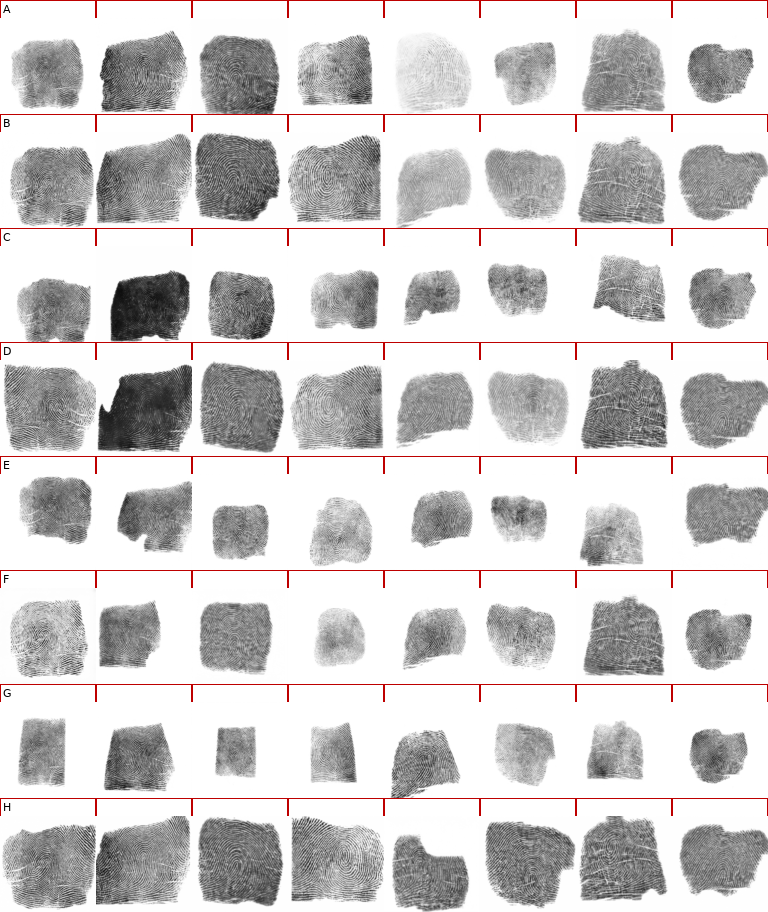
\includegraphics[width=\linewidth]{figures/qc_sensor_overview.png}
    \caption{QC sheet for the current SD302A synthetic dataset.  The dataset
    contains 500 synthetic identities and 10 impressions per identity,
    distributed across SD302A sensors A--H.}
    \label{fig:sensor_overview}
\end{figure*}

\begin{figure*}[t]
    \centering
    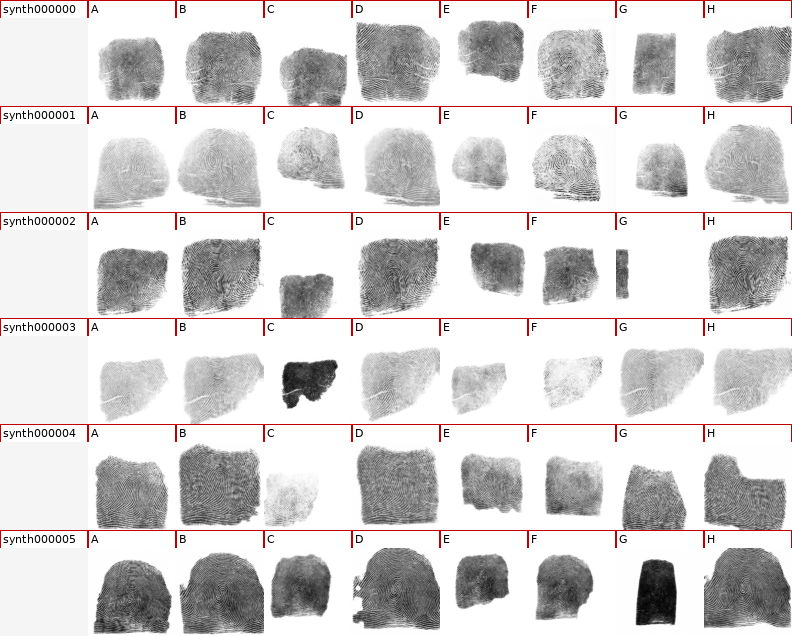
\includegraphics[width=\linewidth]{figures/qc_identity_spread_first6.png}
    \caption{Examples of multiple impressions generated from the same
    synthetic identity under different sensor conditions.  Pose-mask alignment
    reduces the single-pose failure mode observed when the raw identity ridge is
    used directly as the control image.}
    \label{fig:identity_spread}
\end{figure*}

\subsection{Cross-Sensor Extension}

The additional datasets are used to test sensor coverage rather than to claim a
direct FPGAN-Control comparison.  SD301A and SD302B increase the diversity of
contact and rolled sensors used in Stage 1.  FVC 2004 provides compact
benchmarks with sensor styles that differ from SD302A.  Figure~\ref{fig:fvc}
shows an inspection sheet used to identify FVC sensors whose image statistics
are close enough to SD302A-style sensors that ConvNeXt reference conditioning
and Stage-2 LoRA adaptation are likely to work.

\begin{figure}[t]
    \centering
    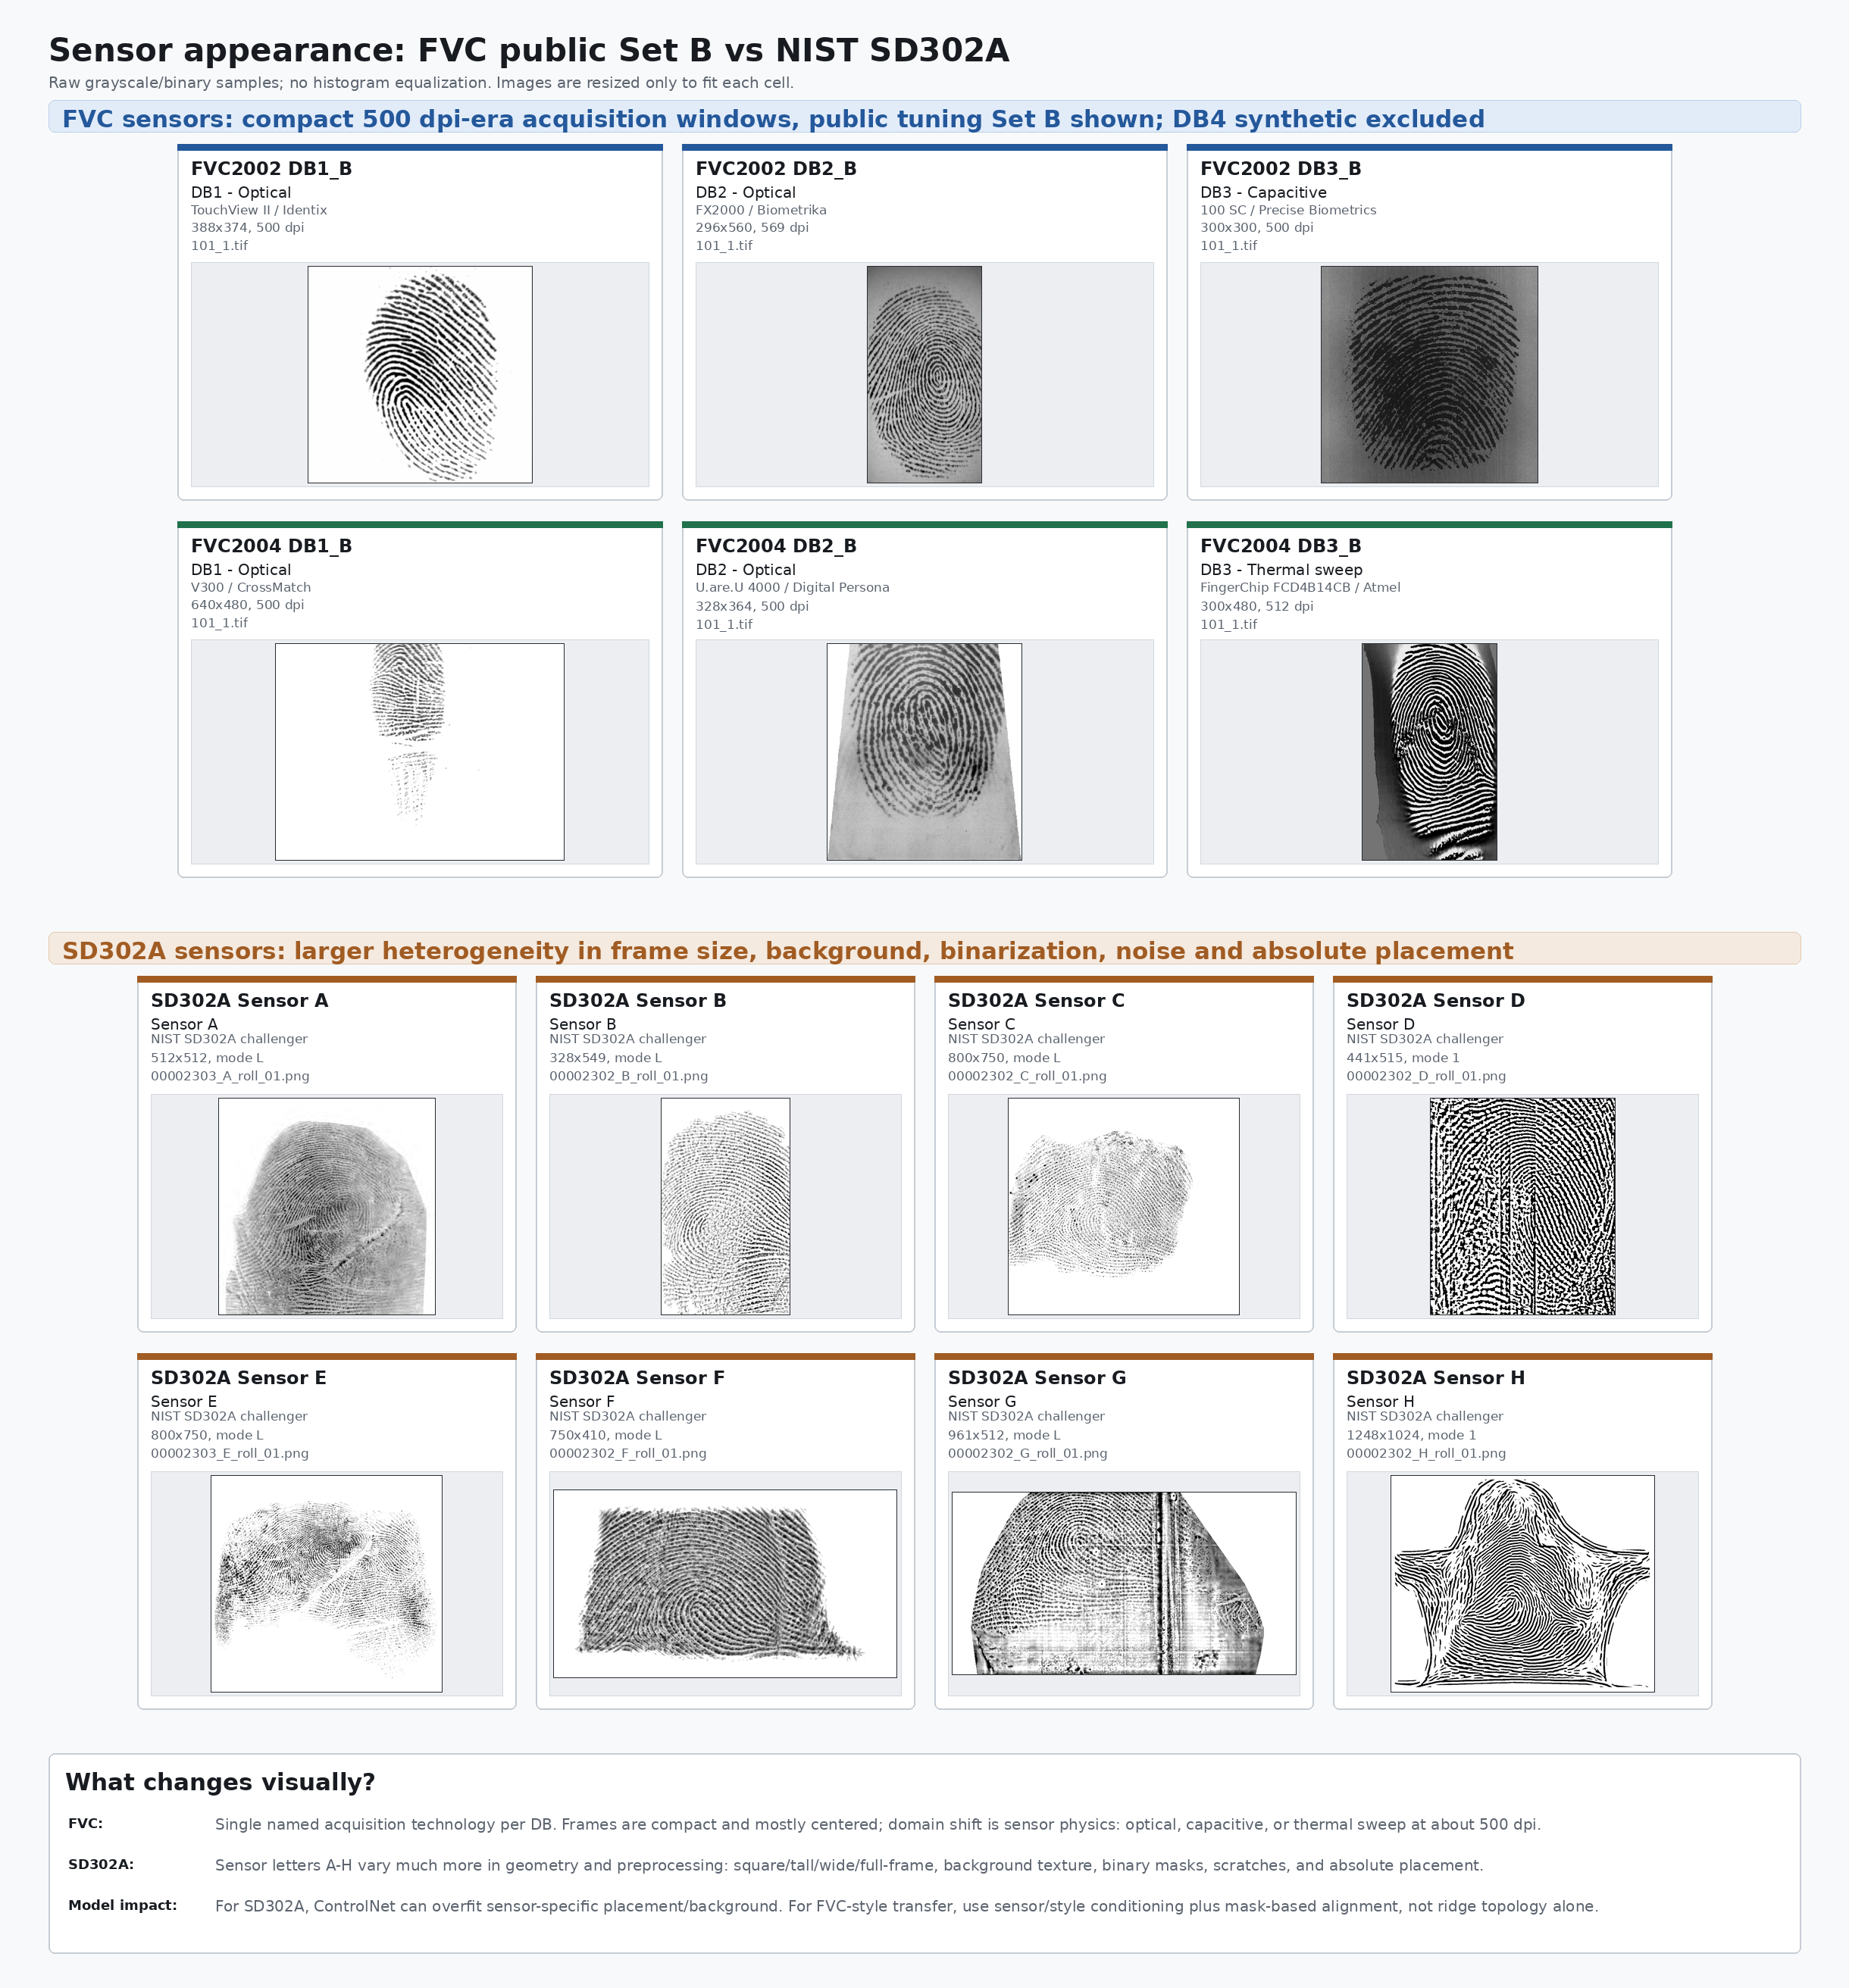
\includegraphics[width=\linewidth]{figures/fvc_vs_sd302a_sensor_comparison.png}
    \caption{Qualitative sensor inspection between FVC and SD302A samples.  We
    use these sheets to select plausible unseen sensors for Stage-2 UNet LoRA
    adaptation.}
    \label{fig:fvc}
\end{figure}

\subsection{Lightweight Design}

The key engineering goal is to make fingerprint synthesis usable by research
groups without large GPU clusters.  Our current Stage-2 TPU training run uses a
compact 64-channel latent UNet and reaches about 7.05 steps/s for global batch
size 256 on TPU v5p-8 after pre-encoding latents, with stable compiled-step
time.  For deployment and sensor adaptation, the important point is that a new
sensor does not require retraining the full generator: only a small Stage-2
UNet LoRA adapter is optimized.  This is lighter than a full Stable
Diffusion-scale multi-dataset training recipe such as GenPrint, while retaining
explicit ridge control for identity preservation.

\begin{table}[t]
    \centering
    \caption{Positioning relative to closely related methods.}
    \label{tab:positioning}
    \begin{tabular}{p{0.22\linewidth}p{0.32\linewidth}p{0.34\linewidth}}
        \toprule
        Method & Strength & Limitation addressed by \method \\
        \midrule
        FPGAN-Control & Strong SD302A controllable baseline & We add lightweight diffusion, reference-image sensor conditioning, and LoRA sensor adapters. \\
        GenPrint & Broad multimodal diffusion and zero-shot style control & We target smaller models and cheaper adaptation for A4000-class labs. \\
        \method & Compact latent diffusion with ridge control & Current recognizer-transfer gap remains the main open issue. \\
        \bottomrule
    \end{tabular}
\end{table}

\section{Limitations}
\label{sec:limitations}

The current synthetic dataset is visually plausible but does not yet transfer
as strongly to real SD302A recognition as desired.  Our internal experiments
suggest that the bottleneck is not only Stage-2 ridge following: the generated
Stage-1 identity ridge may still differ from the real SD302A ridge/minutiae
manifold, and ten impressions generated from one synthetic ridge can be too
structurally similar for recognizer training.  The final report should include
additional minutiae statistics, matcher-based genuine/impostor distributions,
and a reproduced FPGAN-Control comparison under the same recognizer protocol.

\section{Conclusion}
\label{sec:conclusion}

\method is a lightweight fingerprint diffusion pipeline designed for practical
synthetic data generation and sensor adaptation.  It combines a compact
sensor-conditioned latent identity model, ridge-conditioned instance
generation, pose-mask alignment, and Stage-2 UNet LoRA adapters for unseen
sensors.  The method is positioned against FPGAN-Control on SD302A, while
SD301A, SD302B, and FVC-style sensors define the cross-sensor extension.  The
remaining work is to finalize the FPGAN-Control comparison, benchmark A4000
sampling and LoRA fine-tuning cost, and close the observed recognizer-transfer
gap with stronger ridge/minutiae realism metrics.

{
    \small
    \bibliographystyle{ieeenat_fullname}
    \bibliography{main}
}

\end{document}
